\subsection{Wheeled robot Kinematics}
\bi{Non-holonomic} systems \textbf{not integrable}, no inst. move in every direct.
\bi{Wheel constraints} $v_i = \omega_i r_i$ ($r_i$ constraints, (wheel radii))
\begin{itemize}
    \item \textit{Driving straight} all $\vec{v}$ equal (ICR: R.Cent.)
    \item \textit{Turning} Wheel axis must intersect the \bi{Instant Centre of Rotation} (ICR) of vehicle,
          speeds: $v_i \div R_i = \Omega$ ($R_i$ = dist. wheel-ICR; $\Omega$: vehicle rotation rate (around ICR))
\end{itemize}
To compute ICR, use $v_i \div R_i = \Omega$ and similarity (see \ref{sec:classic-stereo}.

Below: $\alpha$, $l$ pos in frame, $\beta$ rot at that pos ($z$-ax).
To compute $\vec{c}$ in $\vec{c} \cdot {_B}\vec{v}_{WB} = \omega$
(For multiple wheels, construct mat. from this)

$c_i = [\sin(\alpha + \beta) \div r, -\cos(\alpha + \beta) \div r, -\cos(\beta) \cdot l \div r]$


\bi{Maneuverability}
\begin{itemize}
    \item Deg. of Mobility: $\delta_m = 3 - $\#constrained directions
    \item Deg. of Steerability: $\delta_s = $\#steerable wheels
    \item Deg. of Maneuverability: $\delta_M = \delta_m + \delta_s$
\end{itemize}

\shade{ForestGreen}{Wheel Configurations}

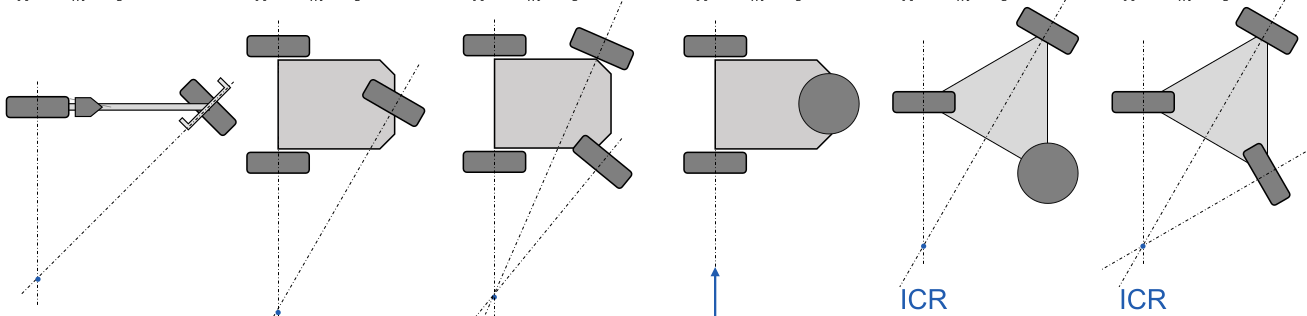
\includegraphics[width=1\columnwidth]{assets/wheel-config.png}

\begin{scriptsize}
    \begin{tabular}{llllll}
        Bicyle         & Tricycle       & Ackermann      & Diff. Drive    & Two-Steer      & Three-Steer    \\
        $\delta_m = 1$ & $\delta_m = 1$ & $\delta_m = 0$ & $\delta_m = 2$ & $\delta_m = 1$ & $\delta_m = 0$ \\
        $\delta_s = 1$ & $\delta_s = 1$ & $\delta_s = 2$ & $\delta_s = 0$ & $\delta_s = 2$ & $\delta_s = 3$ \\
        $\delta_M = 2$ & $\delta_M = 2$ & $\delta_M = 2$ & $\delta_M = 2$ & $\delta_M = 3$ & $\delta_M = 3$ \\
    \end{tabular}
\end{scriptsize}

\subsubsection{Differential Drive Kinematics}
\label{sec:diff-drive-kin}

\bi{State vec} $\vec{x} = [x_1, x_2, \theta]^\top$,
\bi{Inputs} $\vec{u} = [\omega_l, \omega_r]^\top$, wheel radii $r_l, r_r$, $w$ width of robot

\bi{Gen. eq. of Motion} $\dot{x}_1 = v\cos(\theta)$, $\dot{x}_2 = v\sin(\theta)$, $\dot{\theta} = \Omega$,
with $v = 0.5\cdot(\omega_l r_l + \omega_r r_r)$, $\Omega = \frac{\omega_r r_r - \omega_l r_l}{w}$

\textit{Straight}: $v = \omega_l r_l = \omega_r r_r$, $\Omega = 0$, $D = v\Delta t$.

\textit{Turning}: $\Omega = (\omega_l r_l) / R_l\! =\! (\omega_r r_r) / R_r$, $R\! =\! v / \Omega$, $\Delta \theta\! =\! \Omega \Delta t$

\textbf{Discretized}: $\vec{x}_k = \vec{x}_{k - 1} + b_i$ with $i \in \{s, t\}$, respectively, with
$\vec{b}_s = {\scriptsize \begin{bmatrix}
        D \cos(\theta) \\
        D \sin(\theta) \\
        0
    \end{bmatrix}}
    \quad \vec{b}_t = {\scriptsize \begin{bmatrix}
        R(\sin(\Delta \theta + \theta) - \sin(\theta))  \\
        -R(\cos(\Delta \theta + \theta) - \cos(\theta)) \\
        \Delta \theta
    \end{bmatrix}}$; $R$ dist ICR

\textbf{Swedish Wheels}: Have 3 DoF, typ. (3 pcs) equally spaced on circle.
Typ. Param. each: $\alpha, \beta, \gamma$ ($z$, $x$, $y$ axes, oriented along $x$, $z$ up)

\textbf{Wheel rot speed from movement} Typ. comp: $J \cdot \mat{R}(\theta) \cdot \vec{x} = \dot{\varphi}$,
with $\mat{R}(\theta) \cdot \vec{x}$ transform from base frame to robot frame.
% TODO: What's the second Jacobian from?? (See 2017 exam, question B.4)
